% #3599 | Archive/SP_KhoLatex/ID6_old/bai1.2.tex | mã gốc 2H1Y1-2
\begin{vd}%[Đề HK1, SGDDT Quảng Trị 2017]%[Phan Hoàng Anh 12-EX-5]%[2H1Y1-2]
	\immini{Hình đa diện sau có bao nhiêu mặt?
		\motcot
		{$12$}
		{$10$}
		{$6$}
		{\True $11$}}{
		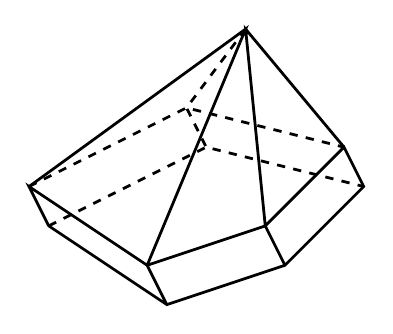
\begin{tikzpicture}[scale=0.5,line width=1]
		\draw(-3,0)--(0,-2)--(3,-1)--(5,1)--(4.5,2)--(2.5,0)--(-0.5,-1)--(-3.5,1)--(-3,0) (-3.5,1)--(2,5)--(-0.5,-1)--(0,-2) (4.5,2)--(2,5)--(2.5,0)--(3,-1);
		\draw[dashed](-3,0)--(1,2)--(5,1) (-3.5,1)--(0.5,3)--(4.5,2) (2,5)--(0.5,3)--(1,2);
		\end{tikzpicture}}
	\loigiai{Hình đa diện đã cho được tạo nên bởi $1$ mặt đáy, $5$ mặt bên ở giữa, $5$ mặt bên ở trên.\\
		Vậy hình đa diện có $11$ mặt.}
\end{vd}

% #3614 | Archive/SP_KhoLatex/ID6_old/DeThamKhao-08.tex | mã gốc 2H1B3-2
\begin{ex}%[Dự án ĐGNL-ĐGTD-2022 GĐ1]%[Thành Đức Trung]%[2H1B3-2]
	Cho khối lăng trụ $ABC.A'B'C'$ có thể tích là $V$. Gọi $M$ là điểm tuỳ ý trên cạnh $AA'$. Thể tích của khối đa diện $M.BCC'B'$ tính theo $V$ là $\dfrac{2V}{k}$, với $k\in\mathbb{N}$. Giá trị của $k$ bằng

	\textit{Kết quả:} \tikz\draw (0,0) rectangle (3,0.6); 
	\loigiai{
		\immini{
			Ta có $\dfrac{V_{MABC}}{V_{A'ABC}}= \dfrac{MA}{AA'}$ và $\dfrac{V_{A'ABC}}{V_{ABC.A'B'C'}}=\dfrac{1}{3}$\\
			nên suy ra $\dfrac{V_{MABC}}{V_{ABC.A'B'C'}} = \dfrac{MA}{3AA'}$.\\
			Chứng minh tương tự ta có $\dfrac{V_{MA'B'C'}}{V_{ABC.A'B'C'}} = \dfrac{MA'}{3AA'}$.\\
			Suy ra $\dfrac{V_{MABC}}{V_{ABC.A'B'C'}} + \dfrac{V_{MA'B'C'}}{V_{ABC.A'B'C'}}  = \dfrac{MA}{3AA'}+ \dfrac{MA'}{3AA'} = \dfrac{1}{3}$.\\
			Do đó $V_{MABC} + V_{MA'B'C'} = \dfrac{1}{3} V_{ABC.A'B'C'}$, từ đó suy ra \\
			$V_{M.BCC'B'} = V_{ABC.A'B'C'} - \left( V_{MABC} + V_{MA'B'C'} \right) = \dfrac{2V}{3}$.\\
			Vậy $k = 3$.
		}{
			\begin{tikzpicture}[scale=0.8,>=stealth,font=\footnotesize, line join=round, line cap=round]
				\tkzDefPoint(0,0){A}
				\tkzDefShiftPoint[A](0:4){C}
				\tkzDefShiftPoint[A](-50:2){B}
				\tkzDefShiftPoint[A](80:4){A'}
				\tkzDefPointsBy[translation = from A to A'](B,C){B',C'}
				\tkzDefPointBy[homothety = center A ratio 0.667](A')\tkzGetPoint{M}
				\tkzDrawPoints(A,B,C,A',B',C',M)
				\tkzDrawSegments(A,A' B,B' C,C' A',B' A',C' B',C' B',M B',C A,B B,C M,B)
				\tkzDrawSegments[dashed](C,M A,C M,C')
				\tkzLabelPoints[right](C',C,B')
				\tkzLabelPoints[left](A,B,A',M)
			\end{tikzpicture}
	}}
\end{ex}

% #3615 | Archive/SP_KhoLatex/ID6_old/DeThamKhao-08.tex | mã gốc 2H1K3-2
\begin{ex}%[Dự án ĐGNL-ĐGTD-2022 GĐ1]%[Thành Đức Trung]%[2H1K3-2]
	Cho lăng trụ $ABCD.A'B'C'D'$ có đáy $ABCD$ là hình thoi cạnh $a$, góc $BAD$ bằng $60^\circ$. Chân đường cao hạ từ $A'$ trùng với tâm $O$ của đáy $ABCD$; Góc giữa mặt phẳng $(AA'B'B)$ với đáy bằng $60^\circ$. Thể tích lăng trụ bằng $\dfrac{3a^3\sqrt{3}}{k}$ với $k\in\mathbb{N}$. Giá trị của $k$ bằng

	\textit{Kết quả:} \tikz\draw (0,0) rectangle (3,0.6); 
	\loigiai
	{
		\immini{	Với giả thuyết ta có tam giác $ABD$ đều cạnh bằng $a$, suy ra diện tích hình thoi $ABCD$ là $S=\dfrac{a^3 \sqrt{3}}{2}$.\\
			Gọi $H$ là hình chiếu của $O$ lên cạnh $AB$, suy ra góc giữa $(AA'B'B)$ với mặt đáy $ABCD$ là góc $A'HO$. Theo đề bài ta có $\widehat{A'HO}=60^{\circ}.$\\
			Xét tam giác $A'HO$, có $OH=\dfrac{a\sqrt{3}}{4}$, $\widehat{A'HO}=60^{\circ}$, suy ra $A'O=\dfrac{3a}{4}$.\\
			Vậy $V_{ABCD.A'B'C'D'}=\dfrac{3a^3 \sqrt{3}}{8}$. Suy ra $k = 8$. 
		}{ \begin{tikzpicture}[scale=0.6, font=\footnotesize, line join=round, line cap=round,>=stealth]
				\tkzDefPoints{-3.4/-2.2/x, 6/0/y, 5.0/6/z, 0/0/B}
				\coordinate (A) at ($(B)+(x)$);
				\coordinate (D) at ($(A)+(y)$);
				\coordinate (C) at ($(D)-(x)$);
				\coordinate (B') at ($(B)+(z)$);
				\coordinate (A') at ($(A)+(z)$);
				\coordinate (D') at ($(D)+(z)$);
				\coordinate (C') at ($(C)+(z)$);
				\tkzInterLL(A,C)(B,D)\tkzGetPoint{O}
				\tkzDefMidPoint(A,B)\tkzGetPoint{I}
				\tkzDefMidPoint(I,B)\tkzGetPoint{H}
				\tkzDrawSegments(A,A' A,D   D,C   C,C' D,D')
				\tkzDrawSegments[dashed](B,A B,C B,D B,B' A,C A',O O,H A',H)
				\tkzDrawPolygon(A',B',C',D')
				\tkzMarkRightAngles(A',O,H O,H,A)
				\tkzLabelPoints[right](C, C', D', D, O)
				\tkzLabelPoints[above](B)
				\tkzLabelPoints[left](A, A', B', H)
				\tkzDrawPoints[fill=black](A,B,C,D,A',B',C',D')
		\end{tikzpicture}}
	}
\end{ex}

% #3617 | Archive/SP_KhoLatex/ID6_old/DeThamKhao-08.tex | mã gốc 2H1K3-2
\begin{ex}%[Dự án ĐGNL-ĐGTD-2022 GĐ1]%[Thành Đức Trung]%[2H1K3-2]
	Cho hình chóp $S.ABC$ có đáy $ABC$ là tam giác vuông tại $B$, $AB=3$, $BC=4$, đường thẳng $SA$ vuông góc với mặt phẳng $(ABC)$, $SA=4$. Gọi $AM$, $AN$ lần lượt là chiều cao các tam giác $SAB$ và $SAC$. Thể tích khối tứ diện $AMNC$ bằng $\dfrac{128}{k}$ với $k\in\mathbb{N}$. Giá trị của $k$ bằng

	\textit{Kết quả:} \tikz\draw (0,0) rectangle (3,0.6); 
	\loigiai{
		\immini{
			\begin{itemize}
				\item Ta có $AM \perp (SBC)$, nên $V_{AMNC}=\dfrac{1}{3} \cdot AM \cdot S_{MNC}$.
				\item Ta có $AM=\dfrac{12}{5}$, $AN=\dfrac{20\sqrt{41}}{41}$, $AC=5$.
				\item $SC \perp (AMN)$, nên tam giác $MNC$ vuông tại $N$. Do đó
				\begin{align*}
					V_{AMNC}=&\dfrac{1}{6} \cdot AM \cdot MN \cdot NC \\
					=& \dfrac{1}{6} \cdot AM \cdot \sqrt{AN^2 - AM^2} \cdot \sqrt{AC^2 - AN^2} \\
					= & \dfrac{128}{41}.
				\end{align*}
			\end{itemize}
		Vậy $k  =41$.
		}{
			\begin{tikzpicture}[scale=1,>=stealth,font=\footnotesize, line join=round, line cap=round]
				\tkzDefPoints{0/0/A,2/-1.5/B,4/0/C,0/4/S}
				\tkzDefPointBy[projection = onto S--B,/tikz/overlay](A) \tkzGetPoint{M}
				\tkzDefPointBy[projection = onto S--C,/tikz/overlay](A) \tkzGetPoint{N}
				\tkzLabelPoints[above](S)
				\tkzLabelPoints[above=2pt,right](N)
				\tkzLabelPoints[below](B)
				\tkzLabelPoints[right](C)
				\tkzLabelPoints[above=2.8pt, left](M)	
				\tkzLabelPoints[left](A)
				\tkzDrawPoints(S,A,B,C,M,N)
				\tkzDrawSegments[dashed](A,C A,N)
				\tkzDrawSegments(S,B A,M M,N C,M)
				\tkzDrawPolygon(S,A,B,C)
				\tkzLabelSegment[below=2pt](B,A){$3$}
				\tkzLabelSegment[below=2pt](C,B){$4$}
				\tkzLabelSegment[midway,left](S,A){$4$}
				\tkzMarkRightAngle[size = 0.2](A,B,C);
				\tkzMarkRightAngle[size = 0.2](A,M,B);
				\tkzMarkRightAngle[size = 0.2](M,N,C);
				\tkzMarkRightAngle[size = 0.2](S,N,A);
				\tkzMarkRightAngle[size = 0.2](A,M,N);
				\tkzMarkRightAngle[size = 0.2](S,A,C);
			\end{tikzpicture}
	}}
\end{ex}

% #3618 | Archive/SP_KhoLatex/ID6_old/DeThamKhao-08.tex | mã gốc 2H1B3-2
\begin{ex}%[Dự án ĐGNL-ĐGTD-2022 GĐ1]%[Thành Đức Trung]%[2H1B3-2]
	Tính thể tích $V$ của khối lăng trụ $ABC.A'B'C'$ biết thể tích của khối chóp $C'.ABC$ bằng $1$. 

	\textit{Kết quả:} \tikz\draw (0,0) rectangle (3,0.6); 
	\loigiai{Ta có $V_{ABC.A'B'C'}=3V_{C'.ABC}=3$.}
\end{ex}

% #3619 | Archive/SP_KhoLatex/ID6_old/DeThamKhao-08.tex | mã gốc 2H1K3-2
\begin{ex}%[Dự án ĐGNL-ĐGTD-2022 GĐ1]%[Thành Đức Trung]%[2H1K3-2]
	Cho khối chóp $S.ABCD$ có thể tích bằng $1$, đáy $ABCD$ là hình thang với cạnh đáy lớn là $AD$ và $AD=3BC$. Gọi $M$ là trung điểm của $SA$, $N$ là điểm thuộc cạnh $CD$ sao cho $ND=3NC$. Mặt phẳng $(BMN)$ cắt cạnh $SD$ tại $P$. Thể tích khối chóp $A.MBNP$ bằng $\dfrac{k}{8}$ với $k\in\mathbb{N}$. Giá trị của $k$ bằng

	\textit{Kết quả:} \tikz\draw (0,0) rectangle (3,0.6); 
	\loigiai{
		Gọi $I=BN\cap AD\Rightarrow \dfrac{DI}{BC}=\dfrac{DN}{NC}=3$, vậy $DI=3BC\Rightarrow DI=AD$ hay $D$ là trung điểm của $AI$. Nối $MI\cap SD=P\Rightarrow$ $P$ là trọng tâm tam giác $SAI$, vậy $SP=\dfrac{2}{3}SD$.\\
		\begin{center}
			\begin{tikzpicture}[scale=1, line join = round, line cap = round]
				\tikzset{label style/.style={font=\footnotesize}}
				\tkzDefPoints{0/0/A,1/-2/B,3/-2/C,6/0/D,2.5/4/S}
				\tkzDefMidPoint(S,A) \tkzGetPoint{M}
				\tkzDefBarycentricPoint(C=3,D=1) \tkzGetPoint{N}
				\tkzInterLL(B,N)(A,D) \tkzGetPoint{I}
				\tkzInterLL(M,I)(S,D) \tkzGetPoint{P}
				\tkzDrawSegments(S,A S,B S,C S,P S,N A,B B,C C,N N,I I,P P,N B,M)
				\tkzDrawSegments[dashed](A,D A,N B,N M,P M,N N,D P,D D,I)
				\tkzDrawPoints(S,A,B,C,D,M,N,P,I)
				\tkzLabelPoints[above](S,P) \tkzLabelPoints[left](A,M,B) \tkzLabelPoints[right](I)
				\tkzLabelPoints[below](C,N,D)
				\tkzLabelSegment[below](B,C){$a$} \tkzLabelSegment[below left](A,D){$3a$}
				\tkzLabelSegment[below right](C,N){\scriptsize $h/4$} \tkzLabelSegment[right](N,D){\scriptsize $3h/4$}
			\end{tikzpicture}
		\end{center}
		Do $M$ là trung điểm $AS$ nên $V_{A.MBNP}=V_{S.MBNP}=V_{S.MBN}+V_{S.MNP}$.\\
		Theo định lý về tỉ số thể tích ta có: $V_{S.MBN}=\dfrac{SM}{SA}\cdot V_{S.ABN}=\dfrac{1}{2}V_{S.ABN}$.\\
		$V_{S.MNP}=\dfrac{SM}{SA}\cdot\dfrac{SP}{SD}\cdot V_{S.AND}=\dfrac{1}{2}\cdot \dfrac{2}{3}\cdot V_{S.AND}=\dfrac{1}{3}V_{S.AND}$.\\
		Gọi $h$ là chiều cao của hình thang $ABCD$ và $BC=a$, ta có:\\
		$S_{ABCD}=2ah$, và $S_{AND}=\dfrac{1}{2}\cdot 3a\cdot \dfrac{3}{4}h=\dfrac{9}{8}ah=\dfrac{9}{16}S_{ABCD}$.\\
		$S_{BNC}=\dfrac{1}{2}\cdot a\cdot \dfrac{1}{4}h=\dfrac{1}{8}ah=\dfrac{1}{16}S_{ABCD}\Rightarrow S_{ABN}=\left(1-\dfrac{1}{16}-\dfrac{9}{16}\right)S_{ABCD}=\dfrac{6}{16}S_{ABCD}$.\\
		Vậy $V_{S.MBN}=\dfrac{1}{2}V_{S.ABN}=\dfrac{1}{2}\cdot \dfrac{6}{16}V_{S.ABCD}=\dfrac{3}{16}$.\\
		$V_{S.MNP}=\dfrac{1}{3}V_{S.AND}=\dfrac{1}{3}\cdot \dfrac{9}{16}V_{S.ABCD}=\dfrac{3}{16}$.\\
		Cuối cùng ta có $V_{A.MBNP}=V_{S.MBN}+V_{S.MNP}=\dfrac{3}{8}$.\\
		Vậy $k = 3$.
	}
\end{ex}

% #3627 | Archive/SP_KhoLatex/ID6_old/btbai1.1.tex | mã gốc 2H1Y1-1
\begin{ex}%[Đề TT lần 3, Chu Văn An, Thái Nguyên 2018]%[Bùi Mạnh Tiến]%[2H1Y1-1]
	Trong một khối đa diện thì
	\haicot
	{hai mặt bất kì có ít nhất một cạnh chung}
	{hai cạnh bất kì có ít nhất một điểm chung}
	{hai mặt bất kì có ít nhất một điểm chung}
	{\True mỗi đỉnh là đỉnh chung của ít nhất ba mặt}
	\loigiai
	{
		Trong khối đa diện thì mỗi đỉnh là đỉnh chung của ít nhất ba cạnh nên nó là đỉnh chung của ít nhất ba mặt.
	}
\end{ex}

% #3641 | Archive/SP_KhoLatex/ID6_old/DeThamKhao-01.tex | mã gốc 2H1B3-3
\begin{ex}%[Dự án ĐGNL-ĐGTD-2022 GĐ1]%[Nguyễn Anh Quốc]%[2H1B3-3]
	Cho hình chóp $S.ABCD$ có đáy $ABCD$ là hình bình hành và $AB=2AC=2a$, $BC=a\sqrt{3}$. Tam giác $SAD$ vuông cân tại $S$, hai mặt phẳng $(SAD)$ và $(ABCD)$ vuông góc nhau. Tính thể tích khối chóp $S.ABCD$.\\
\textit{Kết quả:} \tikz\draw (0,0) rectangle (3,0.6);
	\loigiai{
		\immini
		{
			Gọi $I$ là trung điểm $AD$, vì tam giác $SAD$ vuông cân tại $S$ nên $SI \perp AD$ và $SI=\dfrac{AD}{2}=\dfrac{a\sqrt{3}}{2}$.\\
			Hai mặt phẳng $(SAD)$ và $(ABCD)$ vuông góc nhau.\\
			Suy ra $SI \perp (ABCD)$.\\
			Ta có $AB=2AC=2a$, $BC=a\sqrt{3}$ suy ra tam giác $ACB$ vuông tại $C$.\\
			$S_{A B C D}=2S_{\triangle A C B}=A C\cdot B C=a^2\cdot\sqrt{3}$.\\
			Thể tích $V_{S.A B C D}=\dfrac{1}{3}\cdot S_{A B C D}\cdot S I=\dfrac{a^3}{2}$.
		}
		{
			\begin{tikzpicture}[scale=1, font=\footnotesize, line join=round, line cap=round, >=stealth,scale=0.7]
			\def\bc{3.5} 
			\def\ba{2} 
			\def\h{4} 
			\def\gocB{25} 
			\coordinate[label=below left:$D$] (D) at (0,0);
			\coordinate[label=above right:$A$] (A) at (\gocB:\ba);
			\coordinate[label=below:$C$] (C) at (\bc,0);
			\coordinate[label=right:$B$] (B) at ($(C)-(D)+(A)$);
			\coordinate[label=above left:$I$] (I) at ($(A)!1/2!(D)$); % Thay đổi số 1/2 để đổi vị trí điểm H
			\coordinate[label=above left:$S$] (S) at ($(I)+(90:\h)$);
			\draw (D)--(C)--(B)--(S)--cycle (S)--(C);
			\draw[dashed] (A)--(B) (I)--(S)--(A)--(D) (A)--(C);
			\foreach \diem in {A,B,C,D,S,I}	\fill (\diem)circle(1.5pt);
			\newcommand{\gocv}[4][black]{\draw[#1] ($(#3)!5pt!(#2)$)--($(#3)!2!($($(#3)!5pt!(#2)$)!.5!($(#3)!5pt!(#4)$)$)$)--($(#3)!5pt!(#4)$);}
			\gocv{A}{C}{B}
			
\end{tikzpicture}
			
		}
	}
\end{ex}

% #3642 | Archive/SP_KhoLatex/ID6_old/DeThamKhao-01.tex | mã gốc 2H1K3-2
\begin{ex}%[Dự án ĐGNL-ĐGTD-2022 GĐ1]%[Nguyễn Anh Quốc]%[2H1K3-2]
	Cho hình chóp $S.ABCD$ có đáy là hình chữ nhật với $AD=2a$. Tam giác $SAB$ vuông cân tại $S$ và nằm trong mặt phẳng vuông góc với đáy; biết tổng diện tích tam giác $SAB$ và đáy $ABCD$ bằng $\dfrac{33a^2}{4}$. Tính thể tích khối chóp $S.ABCD$.\\
	\textit{Kết quả:} \tikz\draw (0,0) rectangle (3,0.6);
	\loigiai{
		\immini
		{
			Giả sử $AB=x$ $(x>0)$ và gọi $H$ là trung điểm đoạn $AB$.\\
			Suy ra $SH\perp(ABCD)$ và $SH=\dfrac{AB}{2}=\dfrac{x}{2}$.\\
			Ta có $ S_{\triangle SAB}+S_{ABCD}=\dfrac{33a^2}{4}\Leftrightarrow \dfrac{1}{2}\cdot \dfrac{x}{2}\cdot x+x\cdot 2a=\dfrac{33a^2}{4}\Leftrightarrow x^2+8ax-33a^2=0\Leftrightarrow \heva{& x=3a &(N)\\ &x=-11a& (L).} $\\
			Diện tích hình chữ nhật $ABCD$ là $S_{ABCD}=6a^2$.\\
			Chiều cao $SH$ là $SH=\dfrac{3a}{2}$.		
		}
		{
			\begin{tikzpicture}[scale=0.6, font=\footnotesize, line join=round, line cap=round, >=stealth]
			\tkzDefPoints{0/0/A, -2/-2/B, 3/-2/C}
			\coordinate (D) at ($(A)+(C)-(B)$);
			\tkzDefMidPoint(A,B)\tkzGetPoint{H}
			\coordinate (S) at ($(H)+(0,5)$);
			\tkzDrawSegments[dashed](S,A A,B A,D S,H)
			\tkzDrawPolygon(S,C,D)
			\tkzDrawSegments(S,B B,C)
			\tkzLabelPoints[left](A,B)
			\tkzLabelPoints[right](C,D)
			\tkzLabelPoints[above](S)
			\tkzLabelPoints[below right](H)
			\tkzMarkRightAngle(S,H,A)
			\path (D)--(A) node[above,midway,sloped]{$2a$};
			\path (C)--(D) node[below right,midway,sloped]{$x$};
			
\end{tikzpicture}
		}
		\noindent
		Thể tích khối chóp $S.ABCD$ là $V=\dfrac{1}{3}\cdot SH\cdot S_{ABCD}=\dfrac{1}{3}\cdot\dfrac{3a}{2}\cdot 6a^2=3a^3$.
	}
\end{ex}

% #3643 | Archive/SP_KhoLatex/ID6_old/DeThamKhao-01.tex | mã gốc 2H1K3-2
\begin{ex}%[Dự án ĐGNL-ĐGTD-2022 GĐ1]%[Nguyễn Anh Quốc]%[2H1K3-2]
	Khối lăng trụ đứng $ABC.A'B'C'$ có đáy là tam giác đều cạnh $a,$ diện tích tam giác $A'BC$ bằng $\dfrac{a^2}{2}$. Tính thể tích khối lăng trụ $ABC.A'B'C'$.\\
		\textit{Kết quả:} \tikz\draw (0,0) rectangle (3,0.6);
	\loigiai{
		\immini
		{
			Gọi $I$ là trung điểm $BC$.\\
			Tam giác $A'AB$ và tam giác $A'AC$ bằng nhau (c-g-c) nên $A'B=A'C$.\\
			Do đó tam giác $A'BC$ cân tại $A$, suy ra $A'I\perp BC$.\\
			Khi đó $S_{\triangle A'BC}=\dfrac{1}{2}A'I\cdot BC\Rightarrow A'I=\dfrac{2S_{\triangle A'BC}}{BC}=\dfrac{2\cdot\dfrac{a^2}{2}}{a}=a$.\\
			Tam giác $ABC$ đều nên 
			$AI=\dfrac{a\sqrt{3}}{2}.$\\
			Tam giác $A'AI$ vuông tại $A$ nên $$AA'=\sqrt{A'I^2-AI^2}=\sqrt{a^2-\left(\dfrac{a\sqrt{3}}{2}\right)^2}=\dfrac{a}{2}.$$
			Ta có 
			$V_{ABC.A'B'C'}=S_{\triangle ABC}\cdot AA'=\dfrac{a^2\sqrt{3}}{4}\cdot\dfrac{a}{2}=\dfrac{a^3\sqrt{3}}{8}$.
		}
		{
			\begin{tikzpicture}[scale=0.8, line join = round, line cap = round]
			\tikzset{label style/.style={font=\footnotesize}}
			\tkzDefPoints{0/0/A,5.5/0/C,2/-2/B}
			\coordinate (A') at ($(A)+(0,4.5)$);
			\coordinate (I) at ($(B)!0.5!(C)$);
			\tkzDefPointsBy[translation = from A to A'](B,C){B'}{C'}
			\tkzDrawPolygon(A,B,C,C',B',A')
			\tkzDrawSegments(A',C' B',B A',B)
			\tkzDrawSegments[dashed](A,C A',C A',I A,I)
			\tkzDrawPoints(A,C,B,A',B',C',I)
			\tkzLabelPoints[below right](B')
			\tkzLabelPoints[below](B,I)
			\tkzLabelPoints[left](A',A)
			\tkzLabelPoints[right](C',C)
			
\end{tikzpicture}
			
		}
	}
\end{ex}

% #3644 | Archive/SP_KhoLatex/ID6_old/DeThamKhao-01.tex | mã gốc 2H1B3-3
\begin{ex}%[Dự án ĐGNL-ĐGTD-2022 GĐ1]%[Nguyễn Anh Quốc]%[2H1B3-3]
	Nếu kích thước của một khối lập phương tăng lên $k$ lần thì thể tích của nó tăng lên bao nhiêu lần?
	
	\textit{Kết quả:} \tikz\draw (0,0) rectangle (3,0.6);
	\loigiai{
		Gọi $x$ là độ dài cạnh của hình lập phương lúc đầu.
		
		\noindent Suy ra $x'=kx$ là độ dài cạnh hình lập phương lúc sau. Lập tỉ số
		\[\frac{V'}{V}= \frac{(kx)^3}{x^3}=k^3. \]
		\noindent Vậy thể tích khối lập phương tăng lên $k^3$ lần.}
\end{ex}

% #3645 | Archive/SP_KhoLatex/ID6_old/DeThamKhao-01.tex | mã gốc 2H1K3-3
\begin{ex}%[Dự án ĐGNL-ĐGTD-2022 GĐ1]%[Nguyễn Anh Quốc]%[2H1K3-3]
	Cho hình chóp $S.ABC$. Gọi $(\alpha)$ là mặt phẳng đi qua $A$ và song song với $BC$. Mặt phẳng $(\alpha)$ cắt $SB$, $SC$ lần lượt tại $M$, $N$. Tính tỉ số $\dfrac{SM}{SB}$, biết $(\alpha)$ chia khối chóp thành hai phần có thể tích bằng nhau.	
	
\textit{Kết quả:} \tikz\draw (0,0) rectangle (3,0.6);
	\loigiai{
		\immini{
			Vì $(\alpha)$ song song với $BC$ nên $MN\parallel BC$ do đó, $\dfrac{SM}{SB}=\dfrac{SN}{SC}$.\\
			Ta có $$\dfrac{V_{S.AMN}}{V_{S.ABC}}	=\dfrac{SM}{SB}\cdot\dfrac{SN}{SC}\Leftrightarrow \dfrac{1}{2}=\left( \dfrac{SM}{SB}\right) ^2\Leftrightarrow \dfrac{SM}{SB}=\dfrac{\sqrt{2}}{2}.$$
		}
		{\begin{tikzpicture}[scale=0.8,>=stealth, font=\footnotesize, line join=round, line cap=round]
			\clip (-1,-2.5) rectangle (6,4);
			%%%%%%%%%%%%%%%
			\tkzDefPoints{0/0/B,5/0/A,2/-2/C,1/3/S}
			\coordinate (M) at ($(S)!1/2!(B)$);
			\coordinate (N) at ($(S)!1/2!(C)$);
			\tkzDrawSegments(S,B S,C S,A B,C A,C M,N N,A)
			\tkzDrawSegments[dashed](A,B M,N M,A)
			\tkzDrawPoints[fill=black,size=3](A,B,C,S,M,N)
			\tkzLabelPoints[below](A,B,C)
			\tkzLabelPoints[left](N)
			\tkzLabelPoints[above](S)
			\tkzLabelPoints[above left](M)
			
\end{tikzpicture}}	
	}
\end{ex}

% #3647 | Archive/SP_KhoLatex/ID6_old/DeThamKhao-01.tex | mã gốc 2H1K3-3
\begin{bt}%[Dự án ĐGNL-ĐGTD-2022 GĐ1]%[Nguyễn Anh Quốc]%[2H1K3-3]
	Cho hình chóp $S.ABCD$ có đáy $ABCD$ là hình bình hành tâm $O$ có $AB=a, AC =2a$ và $\widehat{BAC}=60^\circ$. Hình chiếu vuông góc của $S$ trên mặt phẳng đáy là trung điểm $I$ của $AO$. Biết góc tạo bởi cạnh bên $SB$ và đáy bằng $60^\circ$. Tính thể tích khối chóp $S.ABCD$.
	\loigiai{
		\immini{
			Ta có $V_{S.ABCD}=2\cdot V_{S.ABC}=\dfrac{2}{3}\cdot S_{ABC}\cdot SI$.\\
			Mà $S_{ABC}=\dfrac{1}{2}\times AB\times AC\times \sin A= \dfrac{a^2\sqrt{3}}{2}$. Xét tam giác $ABI$ có $AB=a, AI=\dfrac{1}{4}\cdot AC=\dfrac{a}{2}\\
			\Rightarrow BI=\sqrt{AB^2 + AI^2 -2\cdot AB\cdot AI\cdot\cos A}=\dfrac{a\sqrt{3}}{2}\\ \Rightarrow SI =\dfrac{3a}{2}$.\\
			Đáp số: $\dfrac{a^3\sqrt{3}}{2}$.
		}
		{
			\begin{tikzpicture}[ line width=1pt, scale=0.7]
				\tkzDefPoints{0/0/A, -3/-2/B, 3/-2/C, 0/5/a}
				\coordinate (D) at ($(A)+(C)-(B)$);
				\coordinate (O) at ($(A)!.5!(C)$);\coordinate (I) at ($(A)!.5!(O)$);
				\coordinate (S) at ($(I)+(a)$);
				\tkzDrawPolygon(S,B,C)
				\tkzDrawPolygon(S,C,D)
				\coordinate (H) at ($(A)!.3!(B)$);
				\coordinate (K) at ($(S)!.7!(H)$);
				%\tkzDrawSegments(A,B')
				\tkzDrawSegments[dashed](B,D A,C S,I A,B A,D S,A I,B)
				\tkzLabelPoints[above](S)
				\tkzLabelPoints[below](B,C,D,O,I)
				\tkzLabelPoints[left](A)
				%		\tkzMarkRightAngle(O,H,B)
				%		\tkzMarkRightAngle(S,O,C)
				\tkzMarkRightAngle(S,I,O)
				%		\tkzMarkRightAngle(O,K,S)
				\tkzMarkAngle(I,B,S)
				%		\tkzMarkAngle[size =0.3,mksize=1](B,A,C)
				%		\tkzMarkAngle[size =0.4,mksize=3](O,H,S)
			
\end{tikzpicture}
		}
	}
\end{bt}

% #3677 | Archive/SP_KhoLatex/ID6_old/bai3.12.tex | mã gốc 2H1K3-2
\begin{vd}%[2H1K3-2]
Cho hình chóp $S.ABC$ có các mặt phẳng $(SAB)$, $(SBC)$, $(SCA)$ đôi một vuông góc với nhau. Diện tích các tam giác $SAB$, $SBC$, $SCA$ lần lượt là $S_1$, $S_2$, $S_3$. Khi đó thể tích của khối chóp $S.ABC$ là $V=\dfrac{\sqrt{2S_1S_2S_3}}{3}$.
\loigiai
{\immini{Ta có $\heva{& (SAB)\cap (SCA)=SA \\ & (SAB)\perp (SBC)\\ & (SCA)\perp (SBC)}\Rightarrow SA\perp (SBC)$.\\
Chứng minh tương tự thì $SB\perp (SCA)$ và $SC\perp (SAB)$.\\
Do đó $SA$, $SB$, $SC$ đôi một vuông góc với nhau.\\
Vậy thể tích khối chóp $S.ABC$ là
\begin{eqnarray*}
V&=&\dfrac{1}{6}\cdot SA\cdot SB\cdot SC\\
&=&\dfrac{1}{3}\cdot\sqrt{2\left(\dfrac{1}{2}\cdot SA\cdot SB\right)\left(\dfrac{1}{2}\cdot SB\cdot SC\right)\left(\dfrac{1}{2}\cdot SC\cdot SA\right)}\\
&=&\dfrac{\sqrt{2S_1S_2S_3}}{3}.
\end{eqnarray*} }{\begin{tikzpicture}[scale=1, font=\footnotesize, line join=round, line cap=round,>=stealth]
\path (0,0)coordinate (S) (3.5,0) coordinate (C) (1,-1) coordinate (B) ($(S)+(0,2.5)$) coordinate (A);
\draw (A)--(S)--(B)--(C)--cycle (A)--(B);
\draw[dashed] (S)--(C);
\foreach \p/\g in {S/180,B/-90,C/0,A/90} \fill[black] (\p) circle(1pt)+(\g:0.3) node{$\p$};
\draw pic[draw, angle radius=0.2cm]{right angle=A--S--B} pic[draw, angle radius=0.2cm]{right angle=A--S--C} pic[draw, angle radius=0.2cm]{right angle=C--S--B};
\end{tikzpicture}}
}
\end{vd}

% #3682 | Archive/SP_KhoLatex/ID6_old/DeThamKhao-03.tex | mã gốc 2H1K3-3
\begin{ex}%[Dự án ĐGNL-ĐGTD-2022 GĐ1]%[Duong Xuan Loi]%[2H1K3-3]
	Cho hình lăng trụ $ABC.A'B'C'$. Gọi $M$, $N$, $P$ lần lượt là các điểm thuộc các cạnh $AA'$, $BB'$, $CC'$ sao cho $AM=2MA'$, $NB'=2NB$, $PC=PC'$. Gọi $V_1$, $V_2$ lần lượt là thể tích của hai khối đa diện $ABCMNP$ và $A'B'C'MNP$. Tính tỉ số $\dfrac{V_1}{V_2}$.
	
	\textit{Kết quả:} \tikz\draw (0,0) rectangle (3,0.6);
	\loigiai{
		\immini{
			Gọi $S$ là diện tích thiết diện của mặt phẳng $(P)$ vuông góc với các cạnh bên hình lăng trụ và cắt tất cả các cạnh bên đó và hình lăng trụ. Khi đó ta có
			$$ V_1=\frac{1}{3}(AM+BN+CP)\cdot S,  V_2=\frac{1}{3}(A'M+B'N+C'P)\cdot S$$
			nên $\dfrac{V_1}{V_2}=1.$
		}{
		\begin{tikzpicture}[scale=1, font=\footnotesize, line join=round, line cap=round,>=stealth]
			\path
			(0,0)coordinate (A')
			(1.5,-2)coordinate (B')
			(4,0)coordinate (C')
			($(A')+(0.5,3.5)$) coordinate (A)
			($(A)+(B')-(A')$) coordinate (B)
			($(A)+(C')-(A')$) coordinate (C)
			($(A)!2/3!(A')$) coordinate (M)
			($(B')!2/3!(B)$) coordinate (N)	
			($(C)!0.5!(C')$) coordinate (P)		
			;
			\draw (A)--(B)--(C)--(C')--(B')--(A')--cycle (A)--(C) (B)--(B')
			(M)--(N)--(P);
			\draw[dashed] (A')--(C') (M)--(P);	
			\foreach \p/\q in {A/90,B/90,C/90,A'/180,B'/-90,C'/0,M/180,N/-10,P/0}
			\fill[black] (\p) circle (1.0pt)node[shift={(\q:3mm)}]{$\p$};
		\end{tikzpicture}
		}
	}
\end{ex}

% #3683 | Archive/SP_KhoLatex/ID6_old/DeThamKhao-03.tex | mã gốc 2H1K3-2
\begin{bt}%[Dự án ĐGNL-ĐGTD-2022 GĐ1]%[Duong Xuan Loi]%[2H1K3-2]
	Cho hình lãng trụ đứng $ABC.A'B'C'$ có đáy $ABC$ là tam giác cân tại $C$, cạnh đáy $AB=2a$ và góc $\widehat{ABC}=30^{\circ}$. Mặt phẳng $\left(C'AB\right)$ tạo với đáy $(ABC)$ một góc $60^{\circ}$.
	\begin{listEX}
		\item Tìm giao tuyến của hai mặt phẳng $(C'AB)$ và $(CA'B')$.
		\item Tính thể tích của khối lăng trụ $ABC.A'B'C'$.
		\item Tính khoảng cách giữa hai đường thẳng $AB$ và $CB'$.
	\end{listEX}	  
	\loigiai{
		\begin{enumerate}
			\item Trong $(ACC'A')$, gọi $I=AC'\cap A'C$, trong $(BCC'B')$, gọi $J=BC'\cap B'C$.\\
			Ta có $I=AC'\cap A'C\Rightarrow \heva{& I\in AC'\subset(C'AB) \\ & I\in A'C\subset(CA'B')}\Rightarrow I\in (C'AB)\cap (CAB).\quad(1)$\\
			Lại có $J=BC'\cap B'C\Rightarrow \heva{& J\in BC'\subset(C'AB) \\ & J\in B'C\subset(CA'B')}\Rightarrow J\in (C'AB)\cap (CAB).\quad(2)$\\
			Từ $(1)$ và $(2)$ suy ra $IJ=(C'AB)\cap(CA'B')$.
			\item 
			\immini{
				Gọi $M$ là trung điểm của đoạn thẳng $AB$.\\
			Vì $\triangle ABC$ cân tại $C$ nên $CM\perp AB$.\\
			Mặt khác $CC'\perp AB\Rightarrow AB\perp CC'$.\\
			Ta có $\heva{& (C'AB)\cap(ABC)=AB \\ & C'M\subset (C'AB),C'M\perp AB \\ & CM\subset (CAB),CM\perp AB}$\\ 
			$\Rightarrow \left((C'AB),(CAB)\right)=(C'M,CM)=\widehat{C'MC}=60^\circ$.\\
			Ta lại có $\triangle BCM$ vuông tại $M$ và $\widehat{ABC}=30^{\circ}$\\
			$\Rightarrow CM=BM\tan \widehat{ABC}=a\tan30^{\circ}=\dfrac{a}{\sqrt{3}}$.			
			}{
				\begin{tikzpicture}[scale=1, font=\footnotesize, line join=round, line cap=round,>=stealth]
					\path
					(0,0)coordinate (A)
					(1.4,-1.5)coordinate (C)
					(4,0)coordinate (B)
					($(A)+(0,3.2)$) coordinate (A')
					($(A')+(B)-(A)$)coordinate (B')
					($(A')+(C)-(A)$)coordinate (C')		
					($(A)!0.5!(B)$) coordinate (M)		
					($(A')!0.5!(B')$) coordinate (M')
					($(C)!0.7!(M')$) coordinate (H)	
					($(A')!0.5!(C)$) coordinate (I)	
					($(B')!0.5!(C)$) coordinate (J)			
					;
					\draw (A)--(C)--(B)--(B')--(C')--(A')--cycle (C)--(A')--(B')--(C)--(C')--(A)
					(M')--(C')--(B);
					\draw[dashed] (A)--(B) (H)--(C')--(M)--(C)--(M') (I)--(J);	
					\foreach \p/\q in {A/180,C/-90,B/0,A'/180,C'/180,B'/0,M/80,M'/90,
					H/0,I/180,J/0}
					\fill[black] (\p) circle (1.0pt)node[shift={(\q:3mm)}]{$\p$};
				\end{tikzpicture}
			}\noindent 
			Tam giác $CC'M$ vuông tại $C$ và $\widehat{C'MC}=60^\circ\Rightarrow CC'=CM\tan\widehat{C'MC}=\dfrac{a}{\sqrt{3}}\cdot \tan 60^\circ= a$.\\
			Thể tích khối lăng trụ là $V=\dfrac{1}{3}\cdot CC'\cdot \dfrac{1}{2}\cdot CM\cdot AB=\dfrac{1}{6}\cdot a\cdot \dfrac{a}{\sqrt{3}}\cdot 2a=\dfrac{a^3\sqrt{3}}{9}$.
			\item Ta có $AB\parallel A'B'\Rightarrow AB\parallel (CA'B')$.\\
			Do đó $\mathrm{d}(AB,CB')=\mathrm{d}(AB,(CA'B'))=\mathrm{d}(A,(CA'B'))
			=\mathrm{d}(C',(CA'B'))$.\\
			Gọi $H$ là hình chiếu vuông góc của $C'$ trên $CM'$.\\
			Ta có $\heva{& A'B'\perp CC' \\ & A'B'\perp C'M'}\Rightarrow A'B'\perp (CC'M')\Rightarrow A'B'\perp C'H$.\\
			Do đó $\heva{& C'H\perp A'B' \\ & C'H\perp CM'}\Rightarrow C'H\perp (CA'B')$.\\
			Ta được $\mathrm{d}(C',(CA'B'))=C'H$.\\
			Trong tam giác $CC'M'$ vuông tại $C'$, $C'H$ là chiều cao nên
			\[C'H=\dfrac{C'C\cdot C'M'}{\sqrt{C'C^2+C'M'^2}} =\dfrac{a\cdot \dfrac{a}{\sqrt{3}}}{\sqrt{a^2+\left(\dfrac{a}{\sqrt{3}}\right)^2}}=\dfrac{a}{2}.\]
			Vậy $\mathrm{d}(AB,CB')=\dfrac{a}{2}$.
		\end{enumerate}
	}
\end{bt}

% #3690 | Archive/SP_KhoLatex/ID6_old/DeThamKhao-07.tex | mã gốc 2H1B3-3
\begin{ex}%[Dự án ĐGNL-ĐGTD-2022 GĐ1]%[Dao-V- Thuy]%[2H1B3-3]
	Cho hình chóp $S.ABC$ có chiều cao bằng $9$, diện tích đáy bằng $5$. Gọi $M$ là trung điểm của cạnh $SB$ và $N$ thuộc cạnh $SC$ sao cho $NS=2NC$. Thể tích của khối chóp $A.BMNC$ bằng\\
	\textit{Kết quả:} \tikz\draw (0,0) rectangle (3,0.6);
	\loigiai{
		\immini{
			Từ giả thiết, ta có $\dfrac{SN}{SC}=\dfrac{2}{3}$ và $\dfrac{SM}{SB}=\dfrac{1}{2} $.\\
			Thể tích khối chóp $V_{S.ABC}=\dfrac{1}{3}\cdot 9\cdot 5=15 $.\\
			Ta có $$\dfrac{V_{S.AMN}}{V_{S.ABC}}=\dfrac{SM}{SB}\cdot \dfrac{SN}{SC}=\dfrac{1}{3}\Rightarrow V_{ABMNC}=\dfrac{2}{3}V_{S.ABC}=10.$$
		}
		{
\begin{tikzpicture}[line join = round, line cap = round,>=stealth,font=\footnotesize,scale=1]
				\tkzDefPoints{0/0/A}
				\coordinate (B) at ($(A)+(4,0)$);
				\tkzDefShiftPoint[A](60:4){S}
				\tkzDefShiftPoint[A](-25:3){C}
				\tkzDefMidPoint(S,B)\tkzGetPoint{M}
				\coordinate (N) at ($(S)!.67!(C)$);
				\tkzDrawPolygon(S,A,C,B)
				\tkzDrawSegments(S,C A,N M,N)
				\tkzDrawSegments[dashed](B,A A,M)
				\tkzDrawPoints[fill=black](B,C,A,M,N)
				\tkzLabelPoints[above](S)
				\tkzLabelPoints[above right](M)
				\tkzLabelPoints[below](C)
				\tkzLabelPoints[left](A)
				\tkzLabelPoints[right](B,N)
\end{tikzpicture}
		}
	}
\end{ex}

% #3691 | Archive/SP_KhoLatex/ID6_old/DeThamKhao-07.tex | mã gốc 2H1K3-3
\begin{ex}%[Dự án ĐGNL-ĐGTD-2022 GĐ1]%[Dao-V- Thuy]%[2H1K3-3]
	Cho tứ diện $ABCD$ có $AB$, $AC$, $AD$ đôi một vuông góc và $AB=6 \mathrm{\, cm}$, $AC=9 \mathrm{\, cm}$, $AD=3 \mathrm{\, cm}$. Gọi $M$, $N $, $P$ lần lượt là trọng tâm của các tam giác $ABC$, $ACD$, $ADB$.  Thể tích của khối tứ diện $AMNP$ bằng bao nhiêu $\mathrm{cm^3}$?\\
	\textit{Kết quả:} \tikz\draw (0,0) rectangle (3,0.6);
	\loigiai{
		\immini{
			Ta có $$V_{ABCD}=\dfrac{1}{6}AB\cdot AC\cdot AD=27.$$
			Do $$S_{\triangle EFG}=\dfrac{1}{4}S_{\triangle BCD}\Rightarrow V_{AEFG}=\dfrac{1}{4}V_{ABCD}=\dfrac{27}{4}.$$
			Ta có $$\dfrac{V_{A.MNP}}{V_{A.EFG}}=\dfrac{AM}{AE}\cdot \dfrac{AN}{AF}\cdot \dfrac{AP}{AG}=\dfrac{2}{3}\cdot \dfrac{2}{3}\cdot \dfrac{2}{3}=\dfrac{8}{27}.$$
			Vậy $ V_{A.MNP}=\dfrac{8}{27}V_{A.EFG}=2 \mathrm{\, cm^3}$.
		}
		{
\begin{tikzpicture}[line join = round, line cap = round,>=stealth,font=\footnotesize,scale=.9]
				\tkzDefPoints{0/0/B}
				\coordinate (B) at (0,0);
				\coordinate (D) at ($(B)+(4,0)$);
				\tkzDefShiftPoint[B](60:4){A}
				\tkzDefShiftPoint[B](-40:1.8){C}
				\tkzDefMidPoint(C,B)\tkzGetPoint{E}
				\tkzDefMidPoint(C,D)\tkzGetPoint{F}
				\tkzDefMidPoint(B,D)\tkzGetPoint{G}
				\tkzCentroid(D,B,A)\tkzGetPoint{P}
				\tkzCentroid(A,B,C)\tkzGetPoint{M}
				\tkzCentroid(D,C,A)\tkzGetPoint{N}
				\tkzDrawPolygon(A,B,C,D)
				\tkzDrawSegments(A,C A,E A,F)
				\tkzDrawSegments[dashed](B,D E,F F,G G,E A,G M,N N,P P,M)
				\tkzDrawPoints[fill=black](B,C,A,D,E,F,M,N,P,G)
				\tkzLabelPoints[above](A)
				\tkzLabelPoints[below](C,G)
				\tkzLabelPoints[left](B,M,E)
				\tkzLabelPoints[right](D,F,N,P)
\end{tikzpicture}
		}
	}
\end{ex}

% #3692 | Archive/SP_KhoLatex/ID6_old/DeThamKhao-07.tex | mã gốc 2H1K3-4
\begin{bt}%[Dự án ĐGNL-ĐGTD-2022 GĐ1]%[Dao-V- Thuy]%[2H1K3-4]
	Cho lăng trụ tam giác $ABC.A'B'C'$ có đáy $ABC$ là tam giác đều cạnh $a$, $M$ là trung điểm của $BC$ và $A'M$ vuông góc với $BB'$. Biết hình chiếu vuông góc của điểm $A'$ trên mặt phẳng $(ABC)$ trùng với trọng tâm $G$ của tam giác $ABC$.
\begin{enumerate}
		\item Tính thể tích khối lăng trụ $ABC.A'B'C'$.
		\item Tính khoảng cách giữa hai đường thẳng $AB'$ và $A'C$.
\end{enumerate}
\loigiai
{
\begin{center}
\begin{tikzpicture}[>=stealth,line join=round,line cap=round,font=\footnotesize,scale=.81]
\path
(0,0) coordinate (B)
(1,-1.5) coordinate (A)
(7,0) coordinate (C)
($(B)!.5!(C)$) coordinate (M)
($(A)!2/3!(M)$) coordinate (G)
($(G)+(90:5.5)$) coordinate (A')
($(A')+(B)-(A)$) coordinate (B')
($(A')+(C)-(A)$) coordinate (C')
($(A)!-1!(B)$) coordinate (D)
($(C)!.2!(D)$) coordinate (K)
($(A')!.6!(K)$) coordinate (H)
;
\draw (B)--(D)--(C)--(C')--(B')--(B) (B')--(A)--(A')--(B') (A')--(C') (C)--(A')--(K) (A)--(A')--(D);
\draw[dashed] (B)--(C)--(A)--(M)--(A')--(G)--(K) (G)--(H);
\foreach \p/\g in {A/-150, B/180, C/0, C'/45, B'/150, A'/70, G/-90, M/45, K/-45, H/30, D/-90}
\draw[fill=black] (\p) circle (1pt) node[shift=(\g:3mm)] {$\p$};
\end{tikzpicture}
\end{center}
\begin{enumerate}
	\item Vì $\triangle ABC$ đều với $M$ là trung điểm của $BC$ nên ta có\\
	Diện tích $\triangle ABC$ là $S_{\triangle ABC}= \dfrac{1}{2} AB\cdot AC \sin A = \dfrac{a^2\sqrt{3}}{4}$.\\
	$AM= \sqrt{AB^2-BM^2}= \sqrt{a^2-\dfrac{a^2}{4}}= \dfrac{a\sqrt{3}}{2}$. Suy ra $AG= \dfrac{2}{3}AM= \dfrac{a\sqrt{3}}{3}$, $GM= \dfrac{1}{3}AM= \dfrac{a\sqrt{3}}{6}$.\\
	Mặt khác, vì $A'M\perp BB'$, $BB'\parallel AA'$ nên $A'M \perp AA'$.\\
	Do đó $\triangle AA'M$ vuông tại $A'$.\\
	Suy ra $A'G= \sqrt{AG\cdot GM}= \sqrt{\dfrac{a\sqrt{3}}{3} \cdot \dfrac{a\sqrt{3}}{6}}= \dfrac{a\sqrt{6}}{6}$.\\
	Vậy thể tích khối lăng trụ $ABC.A'B'C'$ là
	\[
	V_{ABC.A'B'C'}= \dfrac{a^2\sqrt{3}}{4} \cdot \dfrac{a\sqrt{6}}{6}= \dfrac{a^3\sqrt{2}}{8}.
	\]
	\item Gọi $D$ là điểm đối xứng của $B$ qua $A$, suy ra tứ giác $ADA'B'$ là hình bình hành $\Rightarrow AB' \parallel A'D \Rightarrow AB' \parallel (A'DC)$.\\
	Do đó $\mathrm{d} (AB', A'C)= \mathrm{d} (A, (A'DC))$.\\
	Từ trên ta được $AM \parallel CD \Rightarrow AM \parallel (A'DC) \Rightarrow \mathrm{d} (A, (A'DC))= \mathrm{d}(G, (A'DC))$.\\
	Theo trên ta có $AC= \dfrac{1}{2}{BD}$ suy ra $\triangle BCD$ vuông tại $C$.\\
	Kẻ $GK \perp CD$, $K \in CD$ $\Rightarrow GK \parallel BC$, suy ra tứ giác $GMCK$ là hình chữ nhật.\\
	Gọi $H$ là hình chiếu vuông góc của $G$ trên $A'K$. Ta được $\mathrm{d}(G, (A'CD))=GH$.\\
	Áp dụng hệ thức lượng trong tam giác vuông $A'GK$ ta được
	\[
	GH= \dfrac{GK \cdot A'G}{\sqrt{GK^2+A'G^2}} = \dfrac{\dfrac{a}{2} \cdot \dfrac{a\sqrt{6}}{6}}{\sqrt{\dfrac{a^2}{4}+\dfrac{a^2}{6}}}= \dfrac{a\sqrt{10}}{10}.
	\]
\end{enumerate}
}
\end{bt}

% #3705 | Archive/SP_KhoLatex/ID6_old/DeThamKhao-06.tex | mã gốc 2H1K3-2
\begin{bt}%[Dự án ĐGNL-ĐGTD-2022 GĐ1]%[Bùi Mạnh Tiến]%[2H1K3-2]
	Cho hình lăng trụ $ABC.A'B'C'$ có đáy là tam giác đều. Hình chiếu vuông góc của $A'$ trên mặt phẳng $(ABC)$ là trung điểm của $BC$. Mặt phẳng $(P)$ vuông góc với các cạnh bên và cắt các mặt bên của hình lăng trụ lần lượt tại $D$, $E$, $F$. Biết rằng mặt phẳng $(ABB'A')$ vuông góc với mặt phẳng $(ACC'A')$ và chu vi của tam giác $DEF$ bằng $4$, thể tích của khối lăng trụ $ABC.A'B'C'$ bằng bao nhiêu?
	\loigiai{
		\immini{
			Gọi $M$, $N$ lần lượt là trung điểm của $BC$ và $B'C'$.\\
			Gọi $K$ là giao điểm của $EF$ và $MN$.\\
			Do $\heva{&BC\perp AM\\&BC\perp A'M}\Rightarrow BC\perp (AMNA')\\
			\Rightarrow BC\perp AA'\Rightarrow BC\perp BB'$.\\
			Do $BB'\perp (DEF)$ nên $EF\perp BB'$.\\
			Trong $(BCCB')$ có $EF\perp BB'$ và $BC\perp BB'$ nên $BC\parallel EF$.\\
			Suy ra $K$ là trung điểm $EF$.	
		}
		{
			\begin{tikzpicture}[>=stealth,line cap=round,line join=round,font=\footnotesize,scale=1]
				\path
				(0,0)coordinate(A)++(0:4)coordinate(C)++(210:3)coordinate(B)
				($(B)!.5!(C)$)coordinate(M)++(90:5)coordinate(A')++(0:4)coordinate(C')++(210:3)coordinate(B')
				($(B')!.5!(C')$)coordinate(N)
				($(M)!.45!(N)$)coordinate(K)
				($(B)!.45!(B')$)coordinate(E)
				($(C)!.45!(C')$)coordinate(F)
				($(A)!(M)!(A')$)coordinate(H)
				($(A)!(K)!(A')$)coordinate(D)
				;
				\draw (A')--(B')--(C')--(C)--(B)--(A)--(A')
				(B)--(B') (A')--(C') (M)--(N) (D)--(E)--(F)
				;
				\draw[dashed] (A)--(C) (A')--(M)--(A)
				(M)--(H) (F)--(D)--(K)
				;
				\foreach \x/\g in {A/180,A'/180,C/0,C'/0,B'/90,B/-90,M/-90,D/165,H/165,N/-45,K/-60,E/190,F/10}
				\fill[black](\x)circle(1pt) ($(\x)+(\g:3mm)$)node{$\x$}
				;
			\end{tikzpicture}
		}
		\noindent
		{
			Mặt khác $BC\perp (AMNA')\Rightarrow BC\perp DK\Rightarrow EF\perp DK$.\\
			Xét $\triangle DEF$ có
			\begin{itemize}
				\item $DK$ vừa là đường cao vừa là đường trung tuyến.
				\item $(ABB'A')\perp (ACC'A')$ nên $\widehat{EDF}=90^\circ$.
			\end{itemize}
			Suy ra tam giác $DEF$ vuông cân tại $D$.\\
			Ta có $DE+EF+DF=4\Leftrightarrow \dfrac{EF}{\sqrt{2}}+\dfrac{EF}{\sqrt{2}}+EF=4\Leftrightarrow EF=BC=4\left(\sqrt{2}-1\right)$.\\
			Do tam giác $ABC$ đều nên $AM=\dfrac{BC\sqrt{3}}{2}=2\sqrt{3}\left(\sqrt{2}-1\right)$.\\
			Kẻ đường cao $MH$ của $\triangle AMA'$, suy ra $MH=DK=\dfrac{EF}{2}=2\left(\sqrt{2}-1\right)$.\\
			Xét $\triangle AMA'$ vuông tại $A$ có $\dfrac{1}{MH^2}=\dfrac{1}{MA^2}+\dfrac{1}{MA'^2}\Rightarrow MA'=\sqrt{6}\left(\sqrt{2}-1\right)$.\\
			Vậy thể tích khối lăng trụ $ABC.A'B'C'$ là $V=S_{ABC}\cdot MA'=\dfrac{1}{2}AM\cdot BC\cdot MA'=12\left(10-7\sqrt{2}\right)$.
		}
	}
\end{bt}

% #3709 | Archive/SP_KhoLatex/ID6_old/DeThamKhao-04.tex | mã gốc 2H1K3-2
\begin{ex}%[ĐGNL-ĐGTD-2022, nguyễn hoàng thanh]%[2H1K3-2]
Cho hình lăng trụ đứng $ABC.A'B'C'$ có đáy $ABC$ là tam giác đều cạnh bằng $a$ và $(A'BC)$ hợp với mặt đáy $ABC$ một góc $30^\circ$. Tính thể tích $V$ của khối lăng trụ $ABC.A'B'C'$. \\
\textit{Kết quả:} \tikz\draw (0,0) rectangle (3,0.6);
\loigiai{
\immini{Gọi $M$ là trung điểm của $BC$.\\
Ta có $S_{\triangle ABC}=\dfrac{a^2\sqrt{3}}{4}$.\\
Ta có $\heva{&BC\perp AM\\&BC\perp AA'}\Rightarrow BC\perp (AA'M)\Rightarrow BC\perp A'M$.\\
Suy ra $(A'BC),(ABC))=\widehat{A'MA}=30^\circ$.\\
Xét $\triangle AA'M$ vuông tại $A$, có $AA'=AM\cdot\tan 30^\circ=\dfrac{a\sqrt{3}}{2}\cdot\dfrac{1}{\sqrt{3}}=\dfrac{a}{2}$.\\
Vậy $V_{ABC.A'B'C'}=S_{\triangle ABC}\cdot AA'=\dfrac{a^2\sqrt{3}}{4}\cdot\dfrac{a}{2}=\dfrac{a^3\sqrt{3}}{8}$.
}
{\begin{tikzpicture}[font=\footnotesize, line join=round, line cap=round, >=stealth]
\coordinate  (A) at (0,0);
\coordinate (B) at (4,0);
\coordinate (C) at (2.5,-1.5);
\coordinate[label=right:$M$] (M) at ($(B)!1/2!(C)$);
\coordinate (A') at (0,4);
\coordinate (B') at (4,4);
\coordinate (C') at (2.5,2.5);
\draw (C)--(A')node [above]{$A'$}--(A) (C')node [above]{$C'$}--(A')--(B')node [above]{$B'$}--(B)--(C)node [below]{$C$}--(A) (C)--(C')--(B');
\draw[dashed] (M)--(A)node [below] {$A$}--(B)node [right] {$B$} (M)--(A')--(B);
\tkzDrawPoints[fill=black](A,B,C,A',B',C',M)
\tkzMarkRightAngles[size=.2](C,M,A B,M,A')
\tkzMarkAngles[size=.6,opacity=0.4](A',M,A)
\tkzLabelAngle[pos=1.2](A',M,A){\footnotesize $30^\circ$}

\end{tikzpicture}}
}
\end{ex}

% #3710 | Archive/SP_KhoLatex/ID6_old/DeThamKhao-04.tex | mã gốc 2H1B3-2
\begin{ex}%[ĐGNL-ĐGTD-2022, nguyễn hoàng thanh]%[2H1B3-2]
Thể tích của một khối lập phương là $27$ cm$^3$. Diện tích toàn phần của hình lập phương đó bằng bao nhiêu?\\
\textit{Kết quả:} \tikz\draw (0,0) rectangle (3,0.6);
\loigiai{
Gọi $a$ là cạnh khối lập phương. Vì $a^3=27$ nên $a=3$.\\
Diện tích toàn phần là $6a^2=54$ cm$^2$.
}
\end{ex}

% #3714 | Archive/SP_KhoLatex/ID6_old/DeThamKhao-04.tex | mã gốc 2H1G3-6
\begin{bt}%[ĐGNL-ĐGTD-2022, nguyễn hoàng thanh]%%[2H1G3-6]
	Cho lăng trụ tứ giác đều $ABCD.A'B'C'D'$ có cạnh đáy bằng $1$, chiều cao bằng $x$. Tìm $x$ để góc tạo bởi $AD'$ và $(AB'C')$ đạt giá trị lớn nhất.
	\loigiai{
		\immini{
			Gọi $H$ là hình chiếu vuông góc của $D'$ lên mặt phẳng $(AB'C')$. Khi đó, $AH$ là hình chiếu của $AD'$ lên mặt phẳng $(AB'C')$. Do đó, góc tạo bởi $AD'$ và $(AB'C')$ chính là góc $\alpha = \widehat{D'AH}$.\\
			Ta lại có $\vartriangle D'AH$ vuông tại $H$ nên ta có $\sin{\alpha}=\dfrac{D'H}{AD'}$.\\
			Gọi $V$ là thể tích hình chóp $A.B'C'D'$. Khi đó, ta có
			$$ V=\dfrac{1}{3}AA' \times S_{\vartriangle B'C'D'}=\dfrac{1}{6}x. $$
			Mặt khác, ta có
			\begin{eqnarray*}
				&V&=\dfrac{1}{3}D'H\times S_{\vartriangle AB'C'} =\dfrac{1}{6}D'H \times AB' \times B'C'\\
				& &=\dfrac{1}{6}D'H \times \sqrt{1+x^2}.
			\end{eqnarray*}
			Do đó
			$$ D'H=\dfrac{6V}{\sqrt{1+x^2}}= \dfrac{x}{\sqrt{1+x^2}}.$$
		}
		{\begin{tikzpicture}[scale =1.2,thick]
			\tkzDefPoints{0/0/A, 3/0/D, 1/2/B};
			\tkzDefPointWith[orthogonal,K=1.2](A,D)\tkzGetPoint{A'}
			\tkzDefPointBy[translation = from A to D](B)\tkzGetPoint{C}
			\tkzDefPointBy[translation = from A to D](A')\tkzGetPoint{D'}
			\tkzDefPointBy[translation = from A to B](A')\tkzGetPoint{B'}
			\tkzDefPointBy[translation = from A to B](D')\tkzGetPoint{C'}
			% 					\tkzDefMidPoint(A',C')\tkzGetPoint{I'}
			% 					\tkzDefMidPoint(B',D)\tkzGetPoint{O}
			\tkzDrawSegments(A,A' A',D' D',A A',B' A,D D,C C',B' C,C' D,D' D',C');
			\tkzDrawSegments[dashed](A,B B,C B,B' C',A A,B');
			
			\tkzLabelPoints[left](A',B');
			\tkzLabelPoints[right](C',D');
			\tkzLabelPoints[left](A);
			\tkzLabelPoints[above right](B);
			\tkzLabelPoints[right](D,C)
			
			% 					\tkzMarkAngles[mark=x,size=0.8](B',A,D')
			\end{tikzpicture}}
		Ta lại có $AD'=\sqrt{1+x^2}$. Suy ra
		$$ \sin{\alpha}=\dfrac{x}{\sqrt{1+x^2}\sqrt{1+x^2}}=\dfrac{x}{1+x^2}=\dfrac{1}{x+\dfrac{1}{x}}. $$
		Áp dụng bất đẳng thức Côsi, ta có
		$$ x+\dfrac{1}{x}\ge 2. $$
		Do đó, ta có $\sin{\alpha}\le \dfrac{1}{2}. $\\
		Vì $0 \le \alpha \le 90^\circ$ nên $\alpha$ đạt giá trị lớn nhất khi chỉ khi $\sin{\alpha}$ đạt giá trị lớn nhất, tức là $\sin{\alpha}=\dfrac{1}{2}$ khi
		$$ x=\dfrac{1}{x} \Leftrightarrow x=1. $$
	}
\end{bt}

% #3722 | Archive/SP_KhoLatex/ID6_old/DeThamKhao-05.tex | mã gốc 2H1K3-2
\begin{ex}%[ĐGNL-ĐGTD-2022]%[2H1K3-2]
Cho khối hộp chữ nhật $ABCD .A' B' C' D'$ có đáy là hình vuông, $BD=4 a$, góc giữa hai mặt phẳng $\left(A'BD\right)$ và $(ABCD)$ bằng $30^{\circ}$. Thể tích của khối hộp chữ nhật đã cho bằng bao nhiêu?\\
\fbox{\textbf{Đáp số} $\ldots\ldots\ldots$}
\loigiai{
\immini{
	Vì đáy $ABCD$ là hình vuông nên $BD= AC=4a$ và $BD\perp AC$.\\
	Do đó $S_{ABCD}=\dfrac{1}{2}\cdot AC \cdot BD=\dfrac{1}{2}\cdot 4a \cdot 4a=8a^2.$\\
	Tam giác $A'AO$ vuông tại $A$, ta có $AA'=AO\cdot \tan 30^{\circ}=2a\cdot \dfrac{\sqrt{3}}{3}$.\\
	Vậy thể tích khối hộp chữ nhật là $$V=S_{ABCD}\cdot AA'=8a^2\cdot  2a\cdot \dfrac{\sqrt{3}}{3}=\dfrac{16 \sqrt{3}}{9} a^{3}.$$
}
{
	\begin{tikzpicture}[scale=1, font=\footnotesize, line join=round, line cap=round, >=stealth]
		\def\a{3}
		\path 
		(0:0) coordinate(A) 
		(0:\a) coordinate(B) 
		(-130:{0.55*\a}) coordinate(D) 
		($(B)+(D)-(A)$) coordinate(C);
		\coordinate (O) at ($(B)!0.5!(D)$);
		\foreach \d in {A,B,C,D} \path (\d) + (90:\a) coordinate(\d');
		\draw (A')--(B')--(C')--(D')--cycle (B')--(B)--(C)--(D)--(D') (C)--(C');
		\draw[dashed] (A')--(A) (A)--(B) (A)--(D) (A')--(O) (A)--(C) (B)--(D)--(A')--(B);
		\foreach \d/\g in {A/170, B/0, C/-45, D/-135, A'/150, B'/30, C'/-30, D'/180,O/-90} \fill (\d) circle(1pt) + (\g:.3) node{$\d$};
		\tkzMarkAngles[size=0.4](A',O,A)
		\draw ($(O)+(-0.4,0.5)$) node{$30^{\circ}$};
\end{tikzpicture}}
}
\end{ex}

% #3723 | Archive/SP_KhoLatex/ID6_old/DeThamKhao-05.tex | mã gốc 2H1B3-2
\begin{ex}%[ĐGNL-ĐGTD-2022]%[2H1B3-2]
	Cho tứ diện $SABC$ có các cạnh $SA$, $SB$, $SC$ đôi một vuông góc với nhau. Biết $SA=3 a$, $SB=4a$, $SC=5a$. Tính theo $a$ thể tích $V$ của khối tứ diện $SABC$.\\
\fbox{\textbf{Đáp số} $\ldots\ldots\ldots$}
\loigiai{
	Ta có $\heva{&SA \perp SC \\ & SA \perp SB}$ nên $SA \perp(SBC)$. Suy ra
$$	V_{SABC}=\dfrac{1}{3} \cdot SA \cdot S_{\triangle SBC}=\dfrac{1}{3} \cdot SA \cdot \dfrac{1}{2} \cdot SB \cdot SC=10 a^3 .$$
}
\end{ex}

% #3727 | Archive/SP_KhoLatex/ID6_old/DeThamKhao-05.tex | mã gốc 2H1K3-2
\begin{bt}%[Dự án ĐGNL-ĐGTD-2022 GĐ1]%[Tên GV]%[2H1K3-2]
	Cho lăng trụ $ABC.A'B'C'$ có đáy là tam giác đều cạnh bằng $2$. Hình chiếu vuông góc $A'$ lên mặt phẳng $(ABC)$ trùng với trung điểm $H$ của $BC$. Góc tạo bởi cạnh bên $AA'$ với mặt đáy bằng $45^{\circ}$. Tính thể tích của khối lăng trụ đã cho.
	\loigiai{
		\immini{Ta có $A'H\perp (ABC)$ và $A'A\cap (ABC)=A$ nên góc giữa cạnh bên $AA'$ với mặt đáy là $\widehat{A'AH}=45^\circ$.\\
			Tam giác $ABC$ đều nên $AH$ là đường cao và $$AH=\dfrac{2\sqrt{3}}{2}=\sqrt{3}.$$
			Tam giác $A'HA$ vuông cân tại $H$ nên $A'H=AH=\sqrt{3}$.\\
			Diện tích tam giác đều $ABC$ là $S_{ABC}=\dfrac{2^2\sqrt{3}}{4}=\sqrt{3}$.\\
		}{\begin{tikzpicture}[scale=1, font=\footnotesize, line join=round, line cap=round,>=stealth]
				\path (0,0)coordinate (A) (3,0) coordinate (C) (1,-1) coordinate (B) (0,3) coordinate (h) ($(B)!0.5!(C)$) coordinate (H);
				\foreach \p in {A,B,C} {\draw (\p)--(\p)--+($(H)+(h)$) coordinate (\p');}
				\draw (A')--(B')--(C')--cycle (A)--(B)--(C);
				\draw[dashed] (A')--(H)--(A)--(C);
				\foreach \p/\g in {A/180,B/-90,C/0,A'/150,B'/-30,C'/30,H/-30} \fill[black] (\p) circle(1pt)+(\g:0.3) node{$\p$};
				\tkzMarkAngles[size=0.6cm,arc=l,mark=](H,A,A');
				\tkzLabelAngles[pos=0.9,rotate=0](H,A,A'){$45^\circ$};
				\tkzMarkRightAngles(A',H,A A,H,B);
		\end{tikzpicture}}\noindent
		Vậy thể tích của khối lăng trụ $ABC.A'B'C'$ là $V=S_{ABC}\cdot A'H=\sqrt{3}\cdot\sqrt{3}=3$.
	}
\end{bt}

% #3775 | Archive/SP_KhoLatex/ID6_old/bai3.9.tex | mã gốc 2H1K3-2
\begin{vd}%[2H1K3-2]
	Cho hình chóp tam giác đều $S.ABC$ với $SA = 2a$, $AB = a$. Gọi $H$ là hình chiếu vuông góc của $ A $ trên cạnh $ SC $. Tính thể tích của khối chóp $ S.ABH $ theo $ a $.
	\loigiai{
		\immini{Gọi $ M $ là trung điểm cạnh $ AB $ và $ O $ là tâm của tam giác $ ABC $. Ta có $\heva{&AB \perp CM \\&AB \perp SO} $ nên $ AB\perp (SCM) $, do đó $ AB \perp SC $.\\
		Mặt khác $ SC \perp AH $, suy ra $ SC \perp (ABH) $.\\
		Lại có\\ $ CM = \dfrac{a\sqrt{3}}{2} $, $ OC=\dfrac{a\sqrt{3}}{3} $ nên $ SO = \sqrt{SC^2 - OC^2} = \dfrac{a\sqrt{33}}{3} $.\\
		Do đó $$ MH = \dfrac{SO\cdot CM}{SC}=\dfrac{a\sqrt{11}}{4} \Rightarrow S_{ABH} = \dfrac{1}{2}AB\cdot MH = \dfrac{\sqrt{11}a^2}{8} .$$}
		{\begin{tikzpicture}[line join=round,line cap=round,line width=.6pt,font=\footnotesize,scale=1]
				\coordinate[label=left:$C$] (C) at (0,0);
				\coordinate[label=below left:$B$] (B) at (1,-1);
				\coordinate[label=right:$A$] (A) at (4,0);
				\coordinate[label=below right:$M$] (M) at ($(B)!.5!(A)$);
				\coordinate[label=below:$O$] (O) at ($(C)!2/3!(M)$);
				\coordinate[label=above left:$S$] (S) at ($(O)+(90:4)$);
				\coordinate[label=left:$H$] (H) at ($(C)!2/3!(S)$);
				\draw (C)--(B)--(A)--(S)--cycle (S)--(B)--(H);
				\draw[dashed] (M)--(C)--(A)--(H)--(M) (O)--(S);
				\fill (A)circle(2pt) (B)circle(2pt) (C)circle(2pt) (S)circle(2pt) (O)circle(2pt) (M)circle(2pt) (H)circle(2pt);
		\end{tikzpicture}}
		\noindent Ta có $ SH=SC-HC=SC-\sqrt{CM^2-MH^2} =\dfrac{7a}{4}$.\\
		Do đó, $ V_{S.ABH}=\dfrac{1}{3}\cdot SH\cdot S_{ABH}=\dfrac{7\sqrt{11}a^3}{96} $.
	}
\end{vd}
